\usetikzlibrary{positioning, shapes.geometric, arrows.meta, shadows, calc}

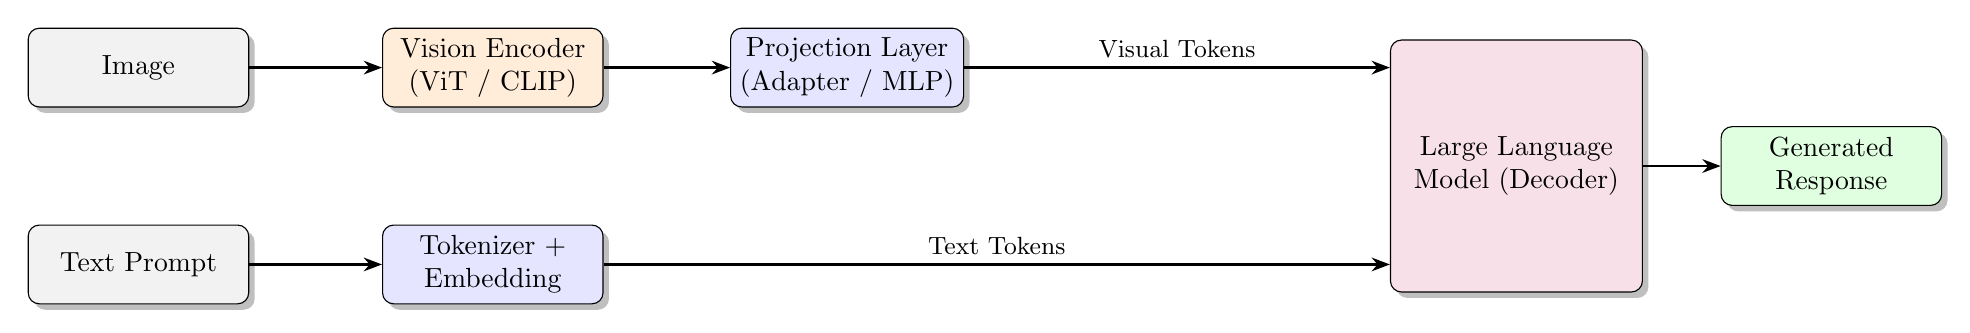
\begin{tikzpicture}[
    block/.style={
        draw,
        rectangle,
        rounded corners,
        minimum width=2.8cm,
        minimum height=1cm,
        align=center,
        drop shadow
    },
    arrow/.style={
        ->,
        >=Stealth,
        thick
    }
]

% Row 1 (y=0): Image processing path
\node[block, fill=gray!10]    at (0,0)   (image) {Image};
\node[block, fill=orange!15]  at (4.5,0) (venc)  {Vision Encoder\\(ViT / CLIP)};
\node[block, fill=blue!10]    at (9,0)   (proj)  {Projection Layer\\(Adapter / MLP)};

% Row 2 (y=-2.5): Text path
\node[block, fill=gray!10]    at (0,-2.5) (text)   {Text Prompt};
\node[block, fill=blue!10]    at (4.5,-2.5) (tokemb) {Tokenizer +\\Embedding};

% LLM block centered between rows
\node[block, fill=purple!12, minimum width=3.2cm, minimum height=3.2cm]
    at (17.5,-1.25) (llm) {Large Language\\Model (Decoder)};

% Output
\node[block, fill=green!12] at (21.5,-1.25) (output) {Generated\\Response};

% Arrows — image path
\draw[arrow] (image) -- (venc);
\draw[arrow] (venc)  -- (proj);
\draw[arrow] (proj.east) -- (llm.west |- proj.east)
    node[midway, above, font=\small] {Visual Tokens};

% Arrows — text path
\draw[arrow] (text) -- (tokemb);
\draw[arrow] (tokemb.east) -- (llm.west |- tokemb.east)
    node[midway, above, font=\small] {Text Tokens};

% Arrow — output
\draw[arrow] (llm) -- (output);

\end{tikzpicture}
